\section{Proposed Methods}


\subsection{Toxicity Detection with KNNs}

This approach is based on the few-shot prompting method for classification.
Few-shot prompting means we provide the model with some examples for the task it is being trained on.
This is a powerful tool used with transformer models to improve their performance significantly.
Research has shown that transformers can utilize their pre-trained knowledge more efficiently when provided with some examples in the prompt.

The downside of few-shot prompting is that the user has to manually add a relevant example in the prompt.
Our approach automates this task to detect toxic content.
We utilize vector databases to find similar toxic and benign examples for a given text.
Moreover, the database is also updated with the latest texts the model identifies during inference, which means the model updates its memory each time it sees a new text.

A vector database stores vector representation of unstructured data.
We have an option to "query" the database with a given vector to find its nearest neighbours or similar vectors.
The vector embeddings for text and image data are formed using encoder-only transformer models.
We use Pinecone as our vector database.

We experiment with different numbers of examples to be extracted from the database and report our results in \autoref{tab:results}.
Below table contains the probabilities of toxicity in text

\begin{table}[h!]
\centering
\begin{tabular}{|c|c|c|c|}
\hline
{\textbf{text}} & \multicolumn{3}{c|}{\textbf{k-shot prompting}} \\ \cline{2-4} 
& \textbf{0 - shot} & \textbf{2 - shot} & \textbf{4 - shot} \\ \hline
I will stab you in the back& 0.99648 & 0.99969 & 0.99972\\ \hline
I will kill animals& 0.98987 & 0.99955 & 0.99970 \\ \hline
you can suck my ... & 0.99685 & 0.99934 & 0.99948 \\ \hline
\end{tabular}
\caption{Toxicity with k-shot prompting}
\label{tab:results}
\end{table}
We can see our approach of k-shot prompting helps us detect the toxicity better.


\subsection{Toxicity-Attended Roberta Classification}
In this approach, we build upon the architecture of the \textit{unitary/unbiased-toxic-roberta} model, introducing key modifications to enhance its focus on offensive content. While the original model features an attention mechanism in its encoder block, we introduce an additional attention layer specifically designed to attend to the context surrounding offensive language (c.f figure \ref{fig:models-diff}).

For this new attention block, we utilize a curated list of profane words from CMU as the \textbf{queries}, while the \textbf{keys} and \textbf{values} are derived from the embeddings of the input text. This mechanism allows the model to selectively focus on the regions of input that contain or are influenced by toxic language, helping it better capture nuanced context around offensive content.

By incorporating this toxicity-attended attention layer, we aim to improve the model's ability to accurately classify toxic and non-toxic content with heightened sensitivity to harmful language patterns.

\begin{figure*}[t] 
    \centering
    \begin{subfigure}[h]{0.47\linewidth} 
        \centering
        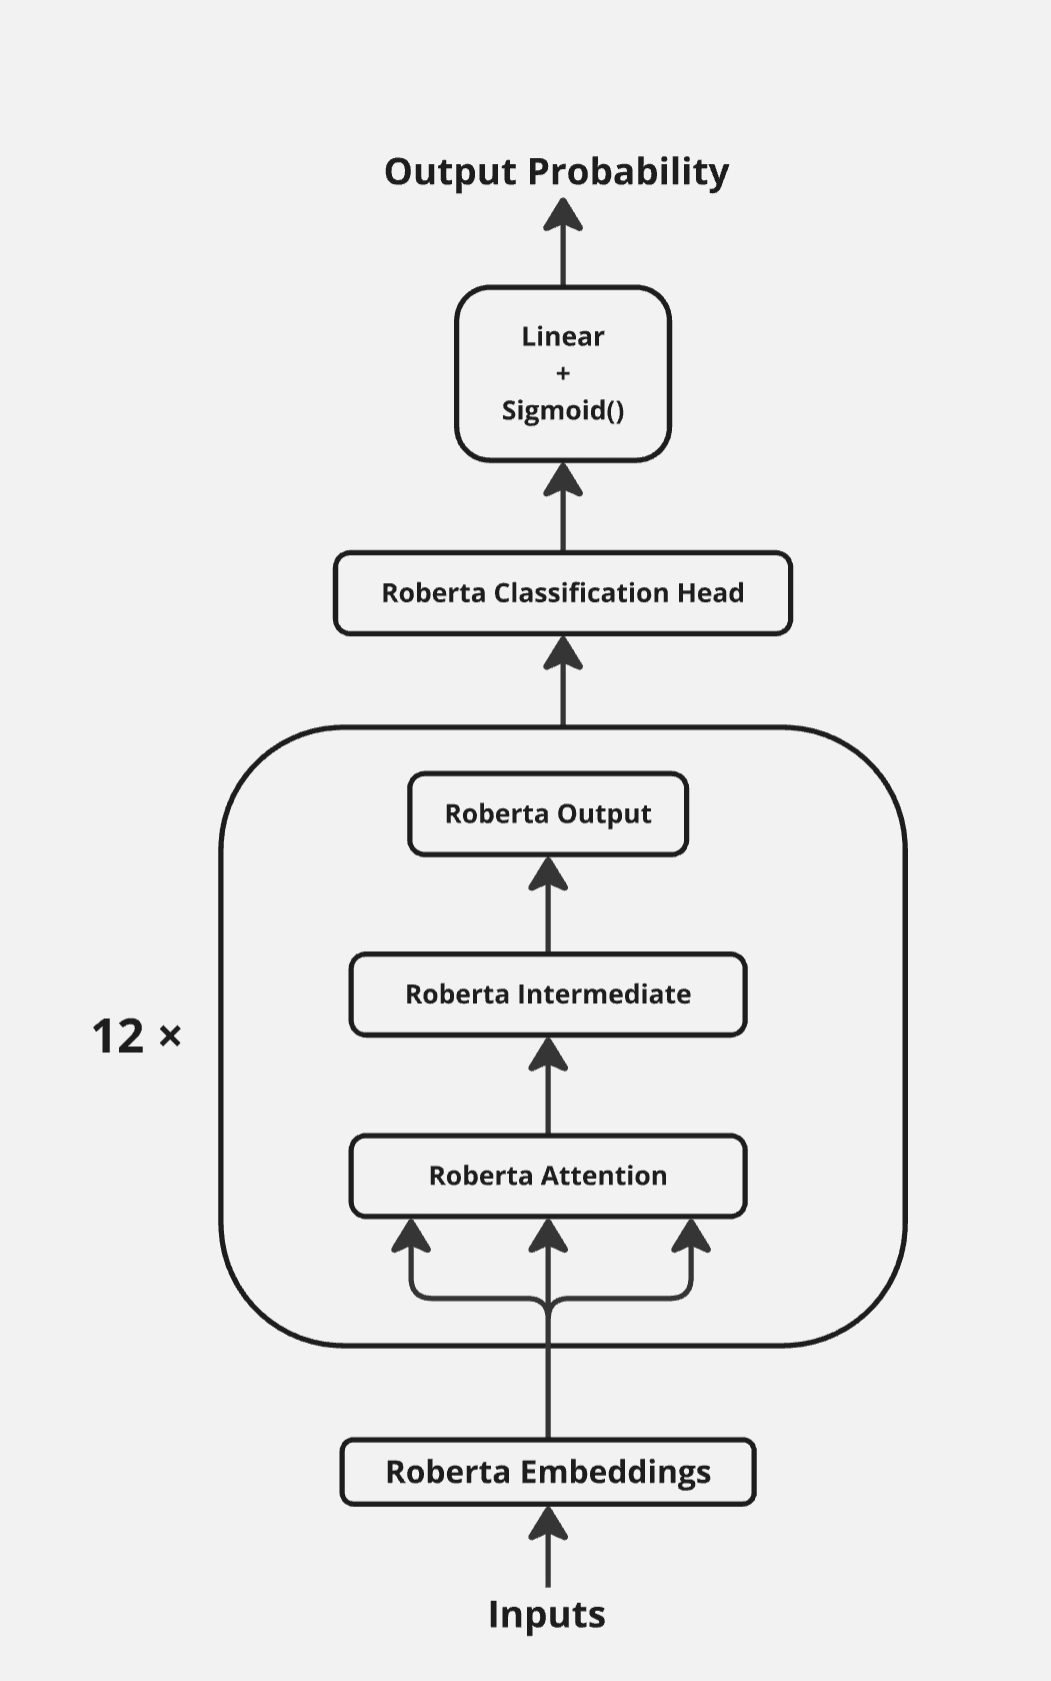
\includegraphics[width=\linewidth]{Images/Screenshot_20241023_113542_Miro.jpg}
        \caption{Original unitary/unbiased-toxic-roberta model}
        \label{fig:org-model}
    \end{subfigure}
    \hspace{0.02\linewidth} % Small space between subfigures
    \begin{subfigure}[h]{0.47\linewidth} 
        \centering
        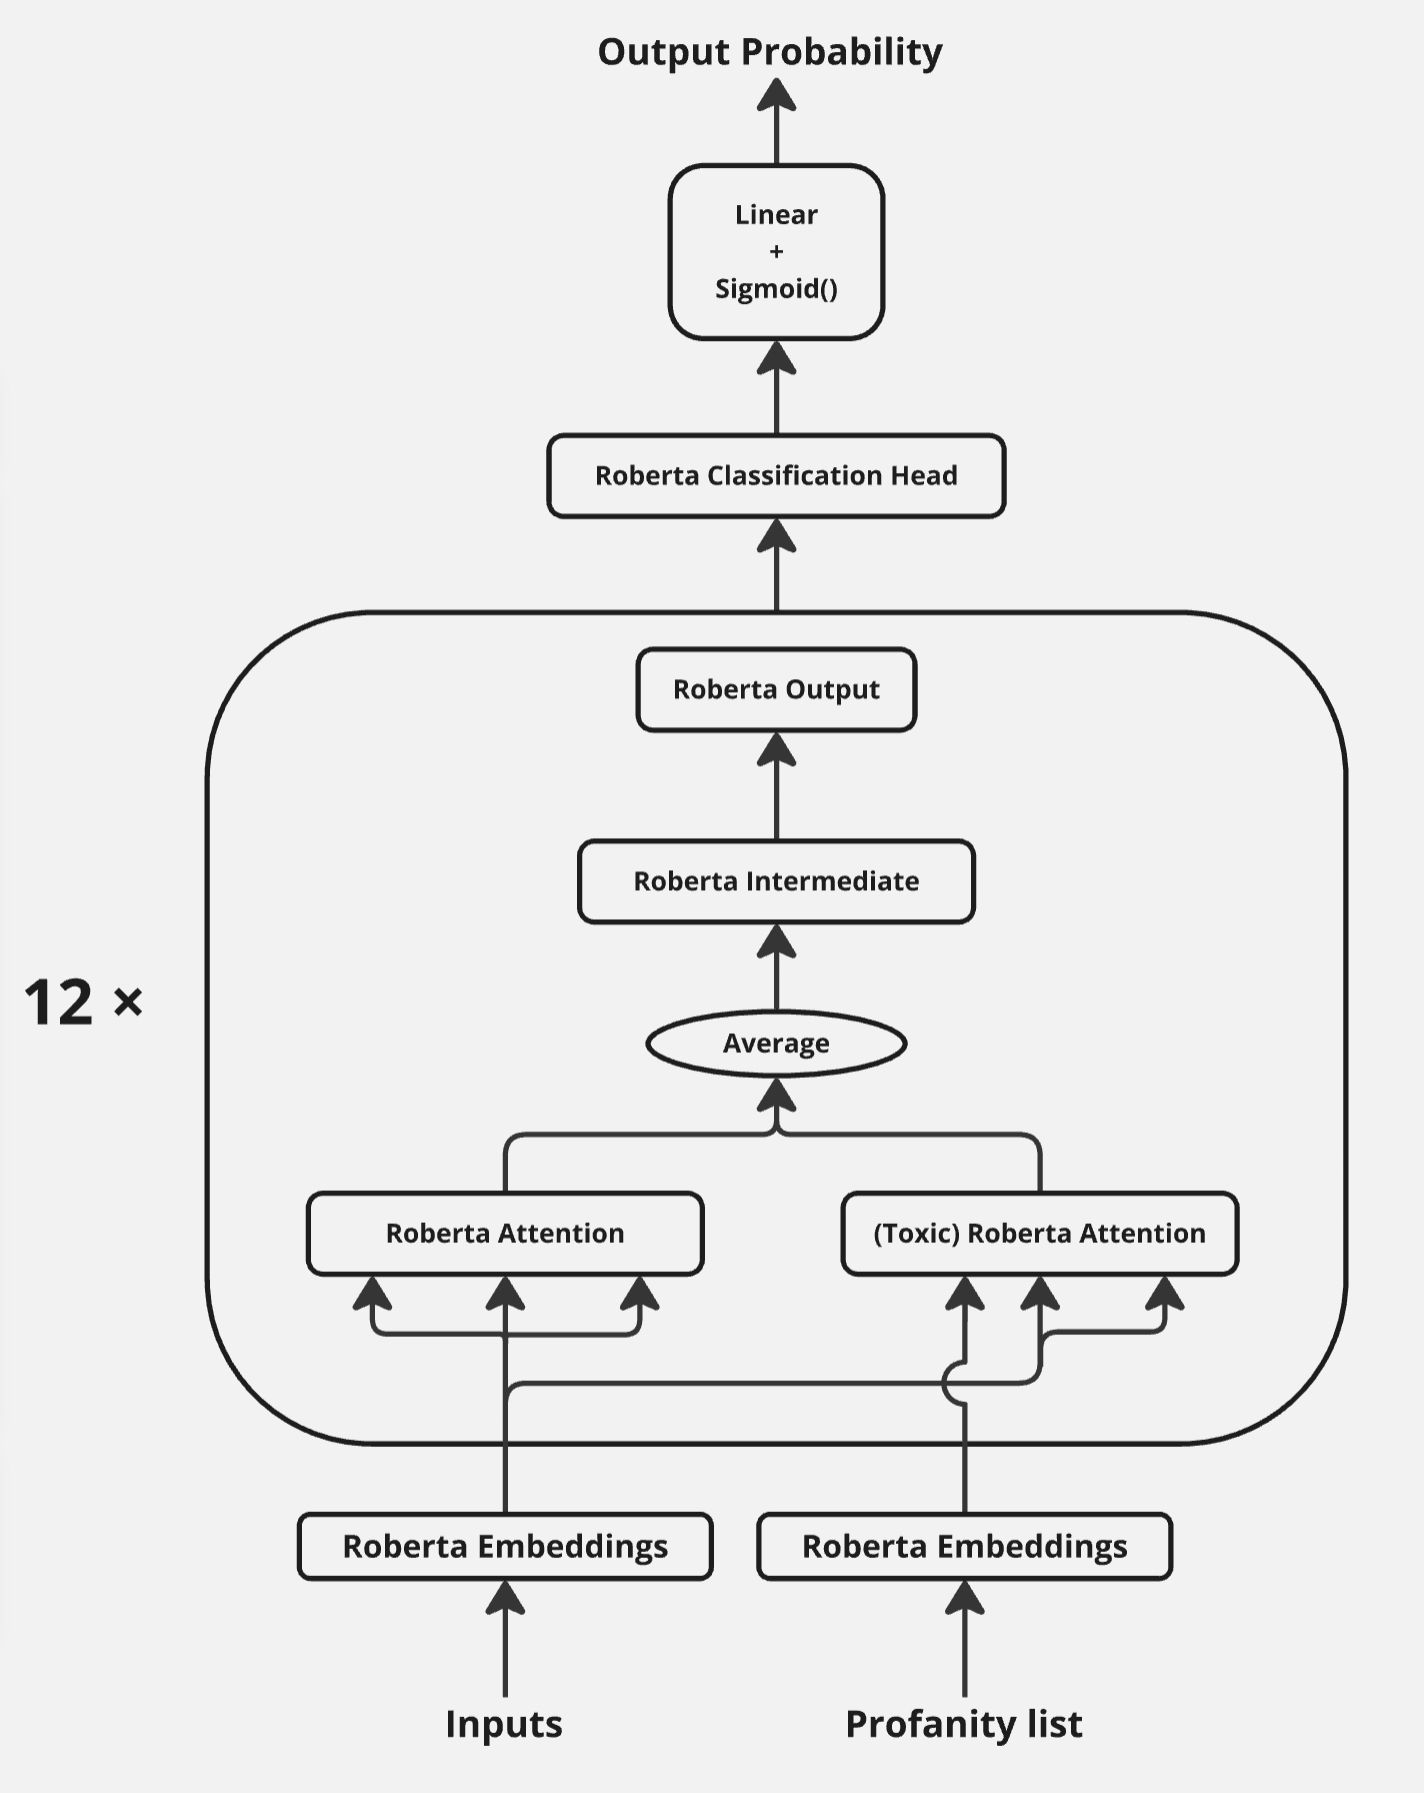
\includegraphics[width=\linewidth]{Images/Screenshot_20241023_113521_Miro.jpg}
        \caption{Toxic-attended roberta model}
        \label{fig:modified-model}
    \end{subfigure}
    \caption{Comparison between the original unitary/unbiased-toxic-roberta model and the modified Toxic-attended Roberta model}
    \label{fig:models-diff}
\end{figure*}




